\problemname{Ljusshow}
Din vän håller på att designa en ljusshow för avslutningsceremonin i årets Programmeringsolympiadsfinal.
Salen där ceremonin hålls kan ses som ett rutnät med $R$ rader och $C$ kolumner.
Utmed de fyra sidorna är olika lampor monterade, vilka kan lysa med en av tre olika färger: rött, blått eller grönt.
Under ceremonin är tanken att lamporna skiftar i olika mönster.

\begin{figure}[h]
    \centering
    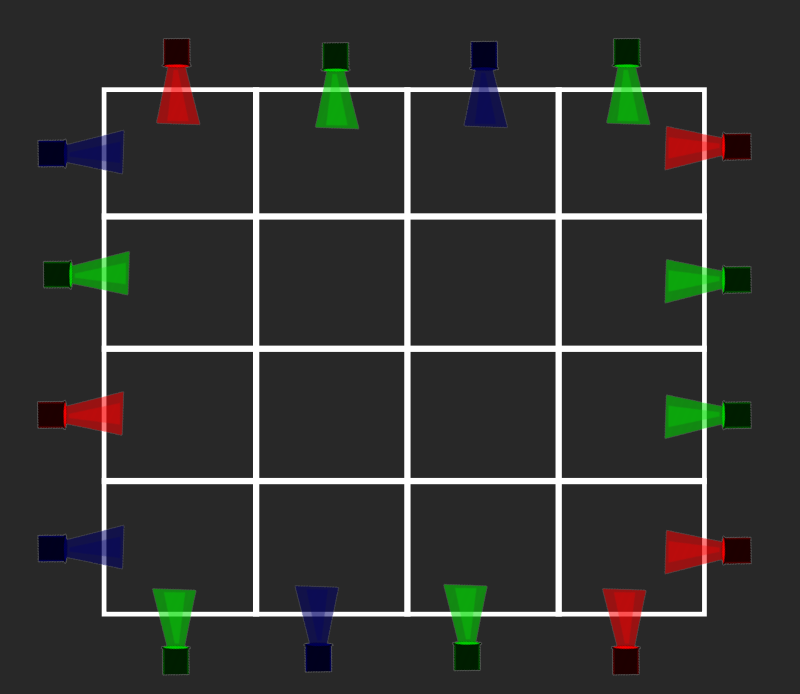
\includegraphics[width=0.6\textwidth]{affischbild}
    \caption{Ett exempel på en konfiguration av lampfärger, där $R = C = 4$. Exemplet motsvarar det enda testfallet som finns i testgrupp 1.}
\end{figure}

En lampa lyser upp samtliga rutor längs med samma kolumn eller rad som den är monterad.
Om en viss ruta lyses upp av minst en lampa av varje färg kommer ljuset i rutan att uppfattas som ett otrevligt bländande vitt.
Din vän har redan designat ett utkast till ljusshowen, och undrar nu om vissa av de valda ljuskonfigurationerna orsakar att för många rutor blir vita.
För att kunna avgöra om en konfiguration är okej eller inte har du fått i uppgift att skriva ett program som läser in vilken färg samtliga lampor ska lysa med, och beräknar antalet rutor som kommer lysa vitt.

\section*{Indata}
Den första raden innehåller två heltal: $R$ ($1 \le R \le 10^6$) och $C$ ($1 \le C \le 10^6$), antalet rader och kolumner i den rutnätsformade salen.

De fyra nästa raderna innehåller en textsträng vardera och beskriver vilka färger alla lampor har.
Den första raden beskriver de $C$ lamporna i toppen av rutnätet som skiner nedåt i ordning vänster till höger,
    den andra de $R$ lamporna i rutnätet till höger om rutnätet som skiner till vänster i ordning uppifrån och ned,
    den tredje de $C$ lamporna under rutnätet som skiner uppåt i ordning vänster till höger,
    den fjärde de $R$ lamporna i rutnätet till vänster om rutnätet som till höger i ordning uppifrån och ned.

Färgen på en lampa beskrivs med hjälp av tecknen \texttt{RGB} beroende på om lampan lyser rött, grönt eller blått.

\section*{Utdata}
Skriv ut ett heltal -- antalet rutor i salen som lyser vitt.
\textbf{Not: svaret ryms inte nödvändigtvis i ett 32-bitars heltal.}

\section*{Poängsättning}
Din lösning kommer att testas på en mängd testfallsgrupper.
För att få poäng för en grupp så måste du klara alla testfall i gruppen.

\noindent
\begin{tabular}{| l | l | p{12cm} |}
  \hline
  Grupp & Poängvärde & Gränser \\ \hline
  $1$    & $20$        &  Gruppen består av ett enda testfall, det som finns på vår affisch (\url{https://www.progolymp.se/2022/affisch.pdf}). \\ \hline 
  $2$    & $15$        &  Alla lampor på samma sida har samma färg. \\ \hline
  $3$    & $25$        &  $R,C \le 1000$ \\ \hline 
  $4$    & $25$        &  Alla lampor till höger eller vänster om rutnätet lyser rött, och alla lampor över och under rutnätet lyser grönt eller blått. \\ \hline
  $5$    & $15$        &  Inga ytterligare begränsningar. \\ \hline
\end{tabular}

\section*{Förklaring av exempelfall}
I det första fallet lyses samtliga rutor på den enda raden upp av rött både från vänster och höger.
Den första rutan lyses upp av grönt både upp- och nedifrån, den andra och fjärde av både grönt och blått, medan den tredje bara lyses upp av blått.
Således är det två av rutorna som lyses upp av alla tre färger och blir vita.

I det tredje exemplet saknas blått ljus helt och hållet.
Därför kan inga rutor vara vita.
